\section{Speculation}
For speculative executions, the first thing for N2O to do is finding the outliers. With the trace log returned by the instrumented processes, N2O use a Kmeans Clustering algorithm, which is commonly used in statistics analysis and data mining, to hunt the outliers. With outliers detected, N2O performs speculative executions, which needs interactive with job scheduler. 

\begin{figure}
\centering
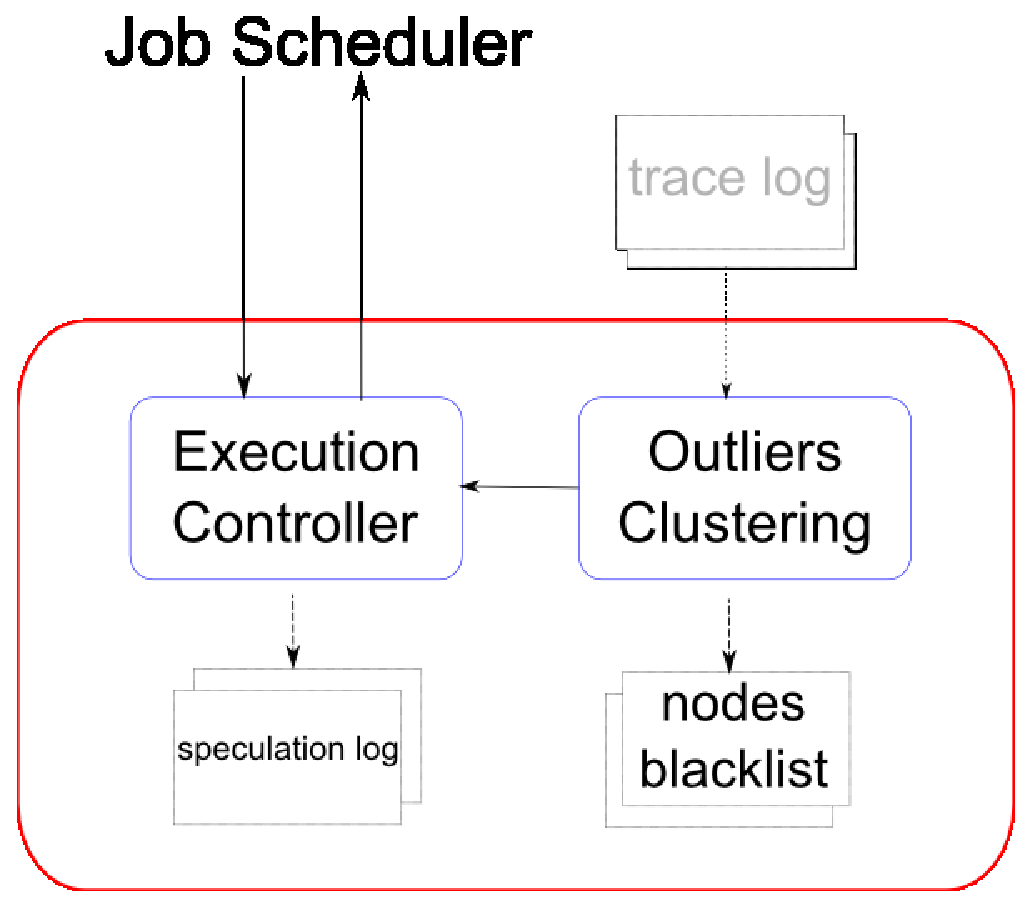
\includegraphics[width=0.62\columnwidth]{figures/speculator.eps}
\caption{Speculator Design}
\label{figure:speculator}
\end{figure}

As shown in Figure 2, two main components, Outliers Clustering and Execution Controller are corresponding to finding outliers and mitigate outliers by speculation. There are several assumptions for the speculator. Outliers is the minority in the massive parallel processes. The tasks is splitted with little imbalance. The server nodes of cluster becomes abnormal indeterminately and may return to normal after a while.

We novelly select two property of each executions to make outliers exposed, the number of tracepoints have been met TPN and the increment of tracepoints TPI in an interval. Figure 3 shows a possible example of two executions of the same binary at runtime, ideally they should draw the same line, but execution B is actually slower than execution A. It is similar to the results in the evaluation with N2O’s instrumenter. 

\begin{figure}
\centering
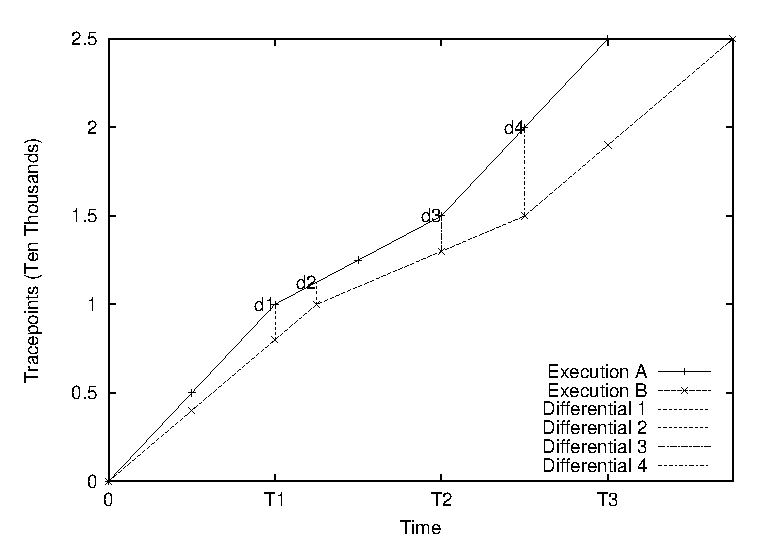
\includegraphics[width=0.62\columnwidth]{figures/executions_example.eps}
\caption{Executions Example}
\label{figure:executionsexample}
\end{figure}

A naive idea for exposing outliers is generating two clustering using a one-degree Kmeans Clustering algorithm, and if the coefficient of variation of the two clusterings’ means is larger than a threshold T, the clustering of executions with a less mean than the other one  will be seen as outliers.

But the number of tracepoints is not increased uniformly. We have proposed this dilemma at the binary instrumentation section. Four differential of two executions’ tracepoints has been marked as d1, d2, d3, d4 at four different time point. Although execution B is always 0.8x slower than execution A, the differential is not increased along the whole timeline. An obvious case is d1 > d2, this may lead to our naive approach mistaken execution B when clustering outliers. Another type of mistake is d3 < d4, execution B may just a little slower than execution A, but seen as an outlier in the naive approach. So there is no fixed threshold is appropriate for detection outliers with the naive idea.

To eliminate  the mistake caused by false positive and false negative, A improved approach has been come up with. We adjustment the threshold T multiplied by normalized mean of TPI of all executions. As one of the assumptions is outliers is minority, the mean of TPI of all executions is similar to the majority. This dynamic threshold can adaptive to the unstable increase of tracepoints perfectly.

The speculative execution algorithm for a job is straightforward with a few of heuristics improvement driven by several rules of thumb. These empirical rules are reasonable and verified in testing. The first rule is giving worst guy of outliers more speculation priority. As speculation is not completely free, it is obviously advisable speculation. Making sure of the split task and merge task not executing on irregular nodes is another important rule because of the impossible of exposing outlier with single task. On the other hand, the split and merge phases are always in the critical path of a job. The last one is speculation as soon as possible without irregular nodes. As the goal of speculation is early completion of job, speculation earlier and faster means better opportunity.

We provide an execution controller implementation with ProActive Scheduler which can be interacted with  a control script. It invokes the outliers clustering module to establish outliers detection with updated trace data. Then maintaining a blacklist of nodes, each node in the blacklist has a penalty value. For outliers, generating a urgency job with only the speculative task and submitting in a speculation priority order. The constraints: no speculation on irregular nodes, can be achieved with a selection script and a claim of nodes selection in the job descriptor. The default speculation interval is 1 seconds, means that the interactive with the job scheduler is moderate. And each update of trace information has a little communication traffic, only an integer indicated the number of  tracepoints transmitted. This lightweight implementation is acceptable to the job scheduler and the impact of performance can be ignore.
